本付録では、計測波形とその周波数スペクトルを図\ref{fig:fig15}-\ref{fig:fig18}に
測線毎に計算した平均波形とその周波数スペクトルを図\ref{fig:fig19}-\ref{fig:fig20}
に示す。これらは、計測したままの波形(Butterworth窓関数を作用させる以前の状態)を示した
もので、本文中に示した結果と本節の結果を比較すれば、窓関数を作用させることによって
初動部分の波形や周波数スペクトルの構造が、ほとんど変化していないことを確認することができる。
%--------------------
\begin{figure}[h]
	\begin{center}
	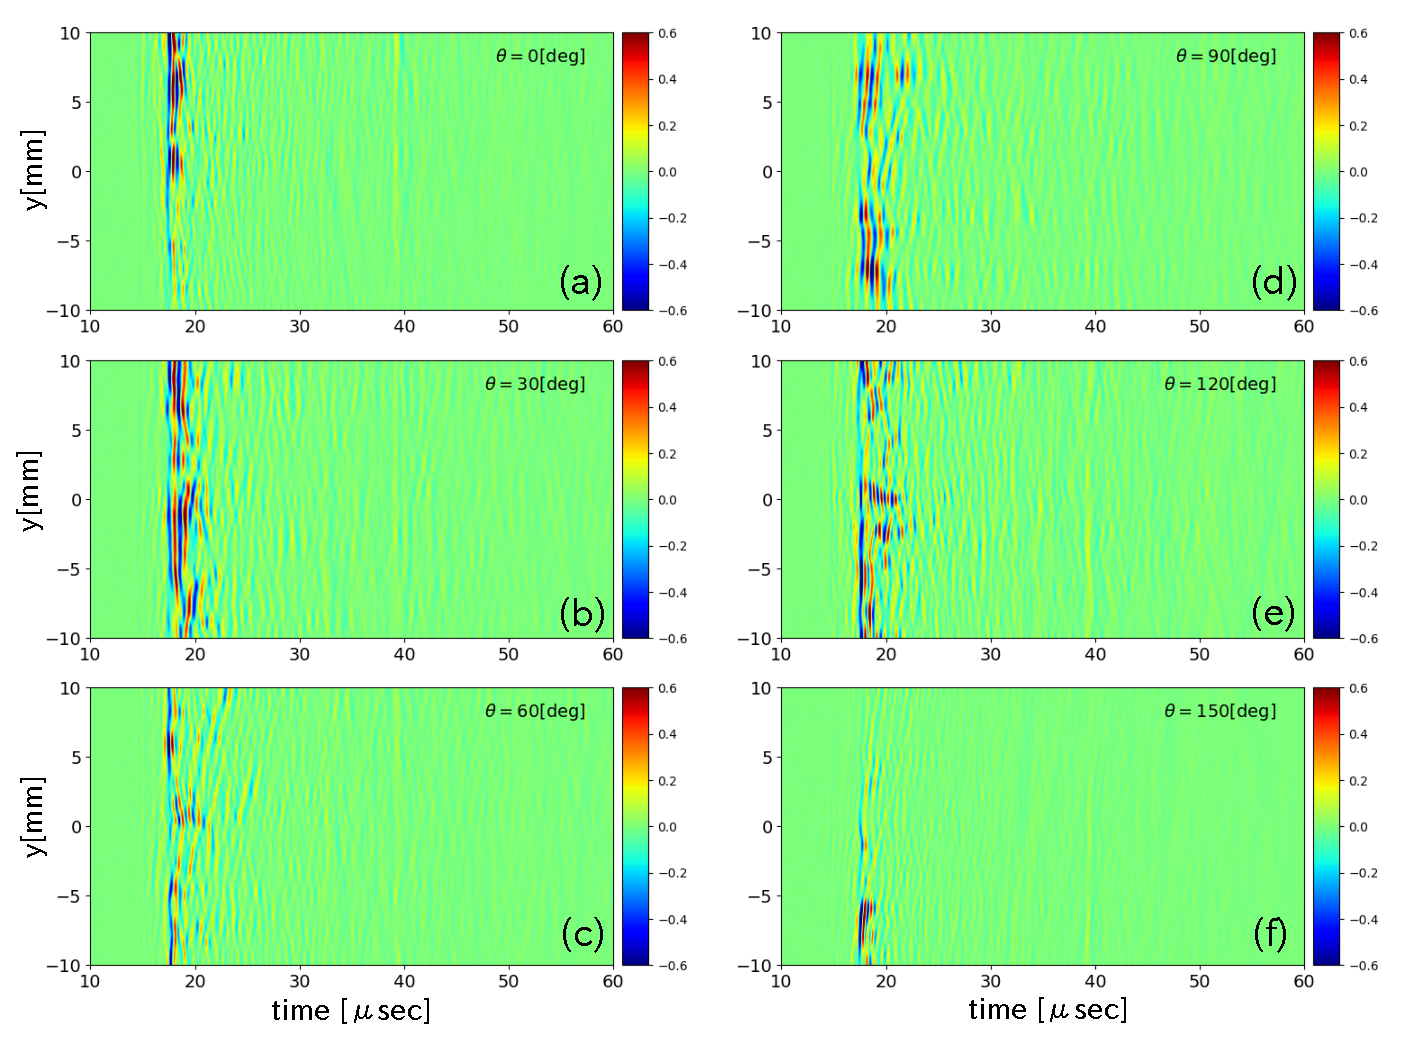
\includegraphics[width=1.0\linewidth]{Figs/fig15.eps} 
	\end{center}
	\caption{
		計測波形の走時プロット($\theta=0\sim 150^{\circ}$).
	} 
	\label{fig:fig15}
\end{figure}
%--------------------
\begin{figure}[h]
	\begin{center}
	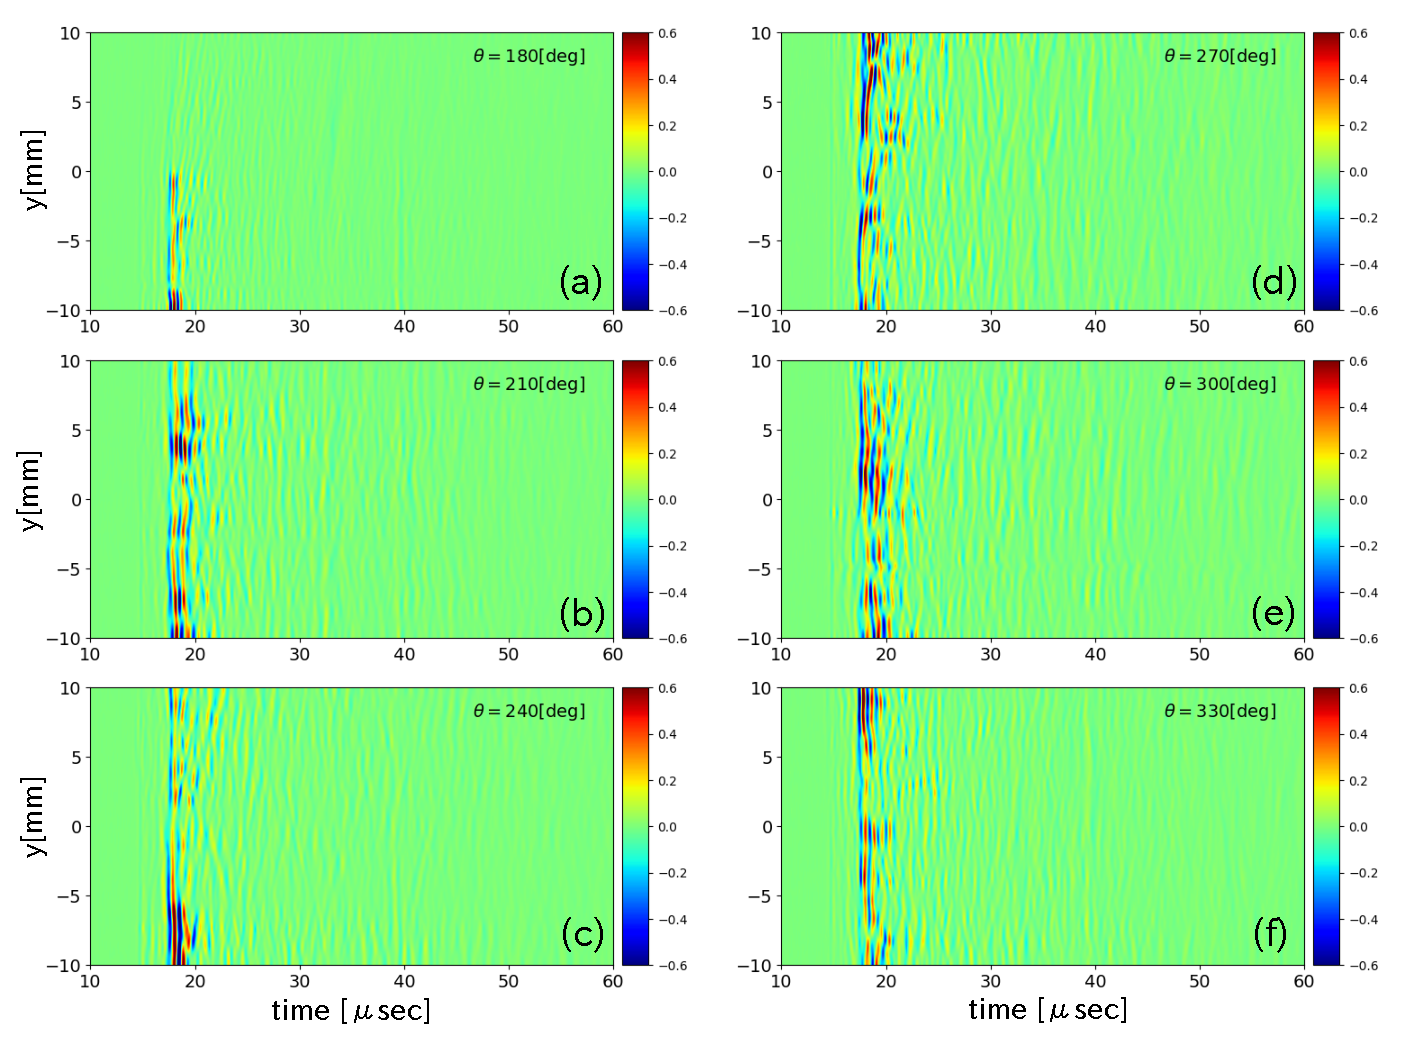
\includegraphics[width=1.0\linewidth]{Figs/fig16.eps} 
	\end{center}
	\caption{
		計測波形の走時プロット($\theta=180\sim 330^{\circ}$).
	} 
	\label{fig:fig16}
\end{figure}
%--------------------
\begin{figure}[h]
	\begin{center}
	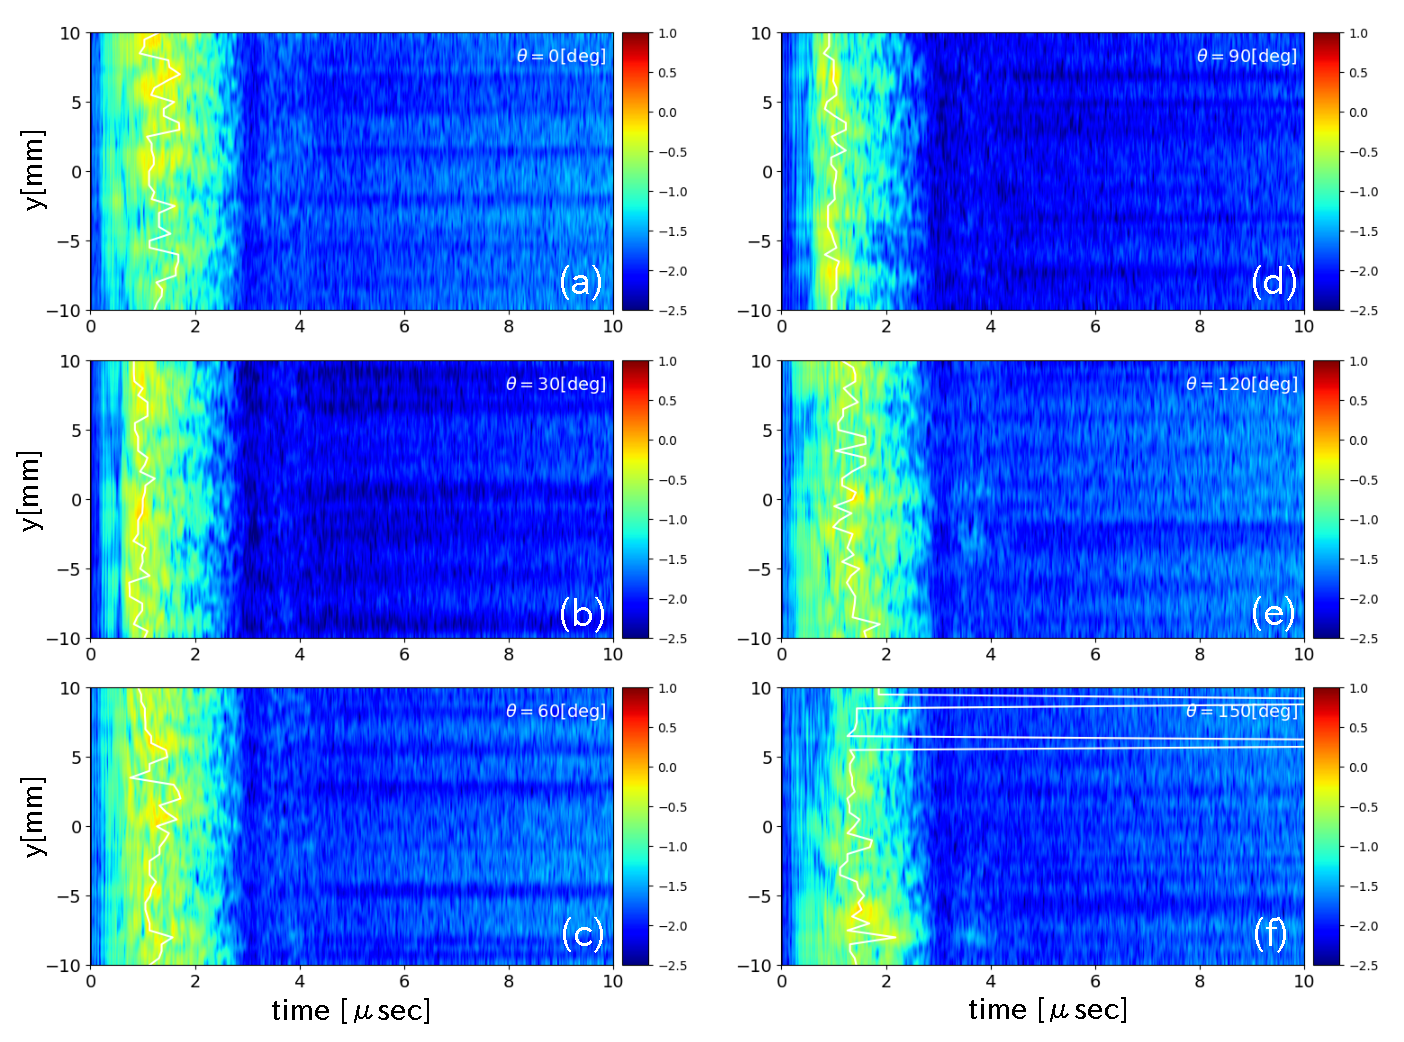
\includegraphics[width=1.0\linewidth]{Figs/fig17.eps} 
	\end{center}
	\caption{
		対数スケールで示した計測波形の周波数スペクトル($\theta=0\sim 150^{\circ}$).
	} 
	\label{fig:fig17}
\end{figure}
%--------------------
\begin{figure}[h]
	\begin{center}
	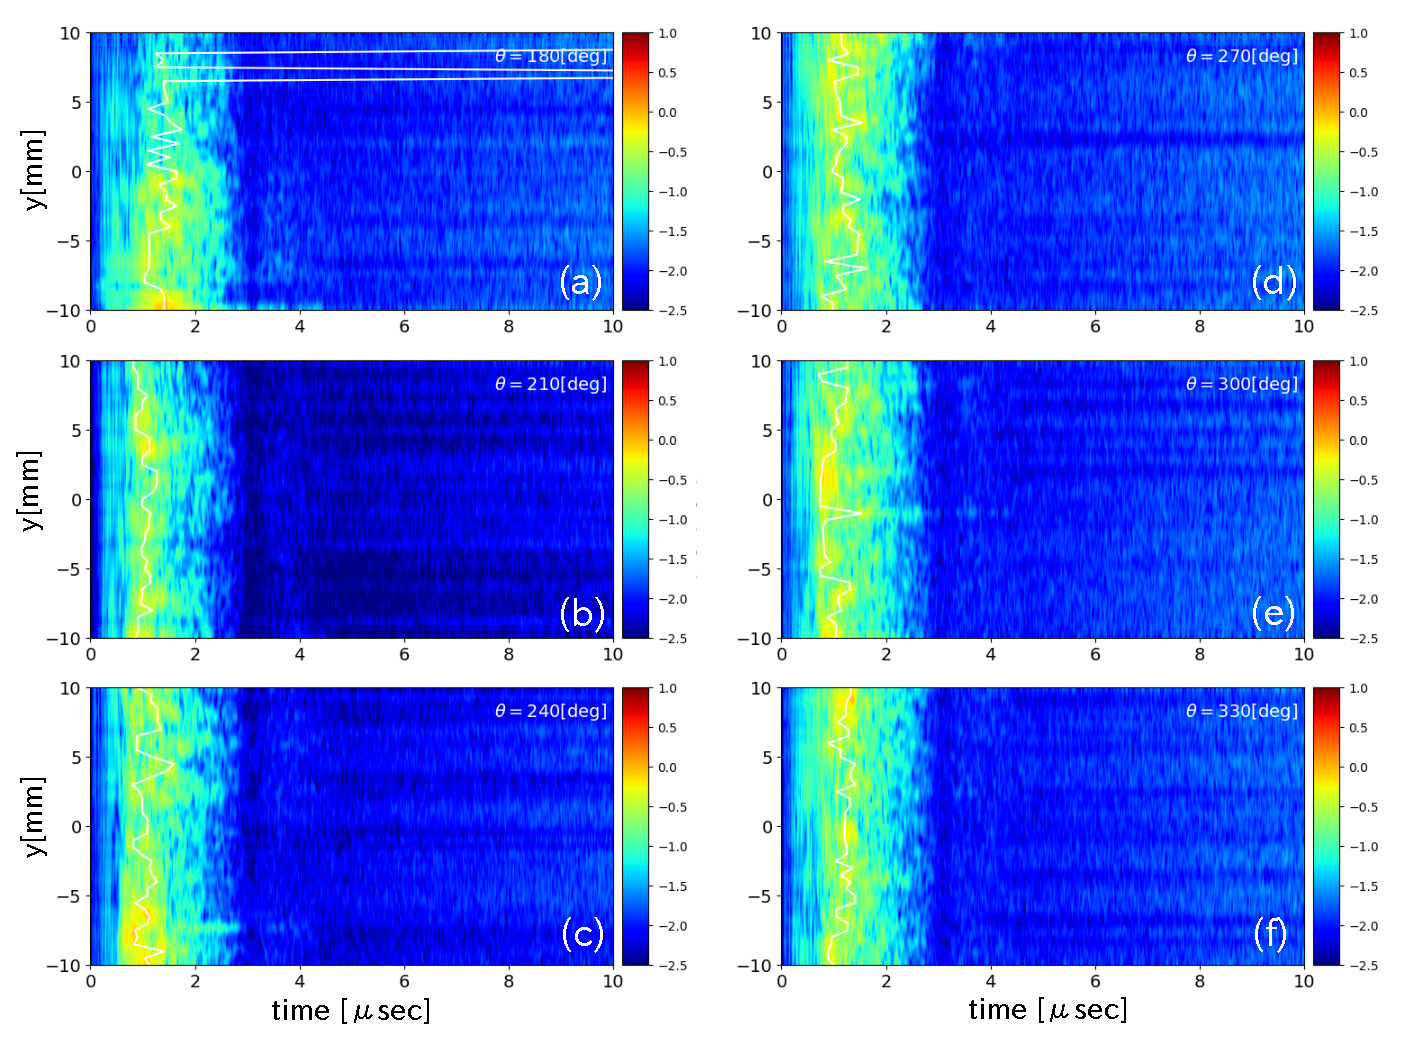
\includegraphics[width=1.0\linewidth]{Figs/fig18.eps} 
	\end{center}
	\caption{
		対数スケールで示した計測波形の周波数スペクトル($\theta=180\sim 330^{\circ}$).
	} 
	\label{fig:fig18}
\end{figure}
%--------------------
\begin{figure}[h]
	\begin{center}
	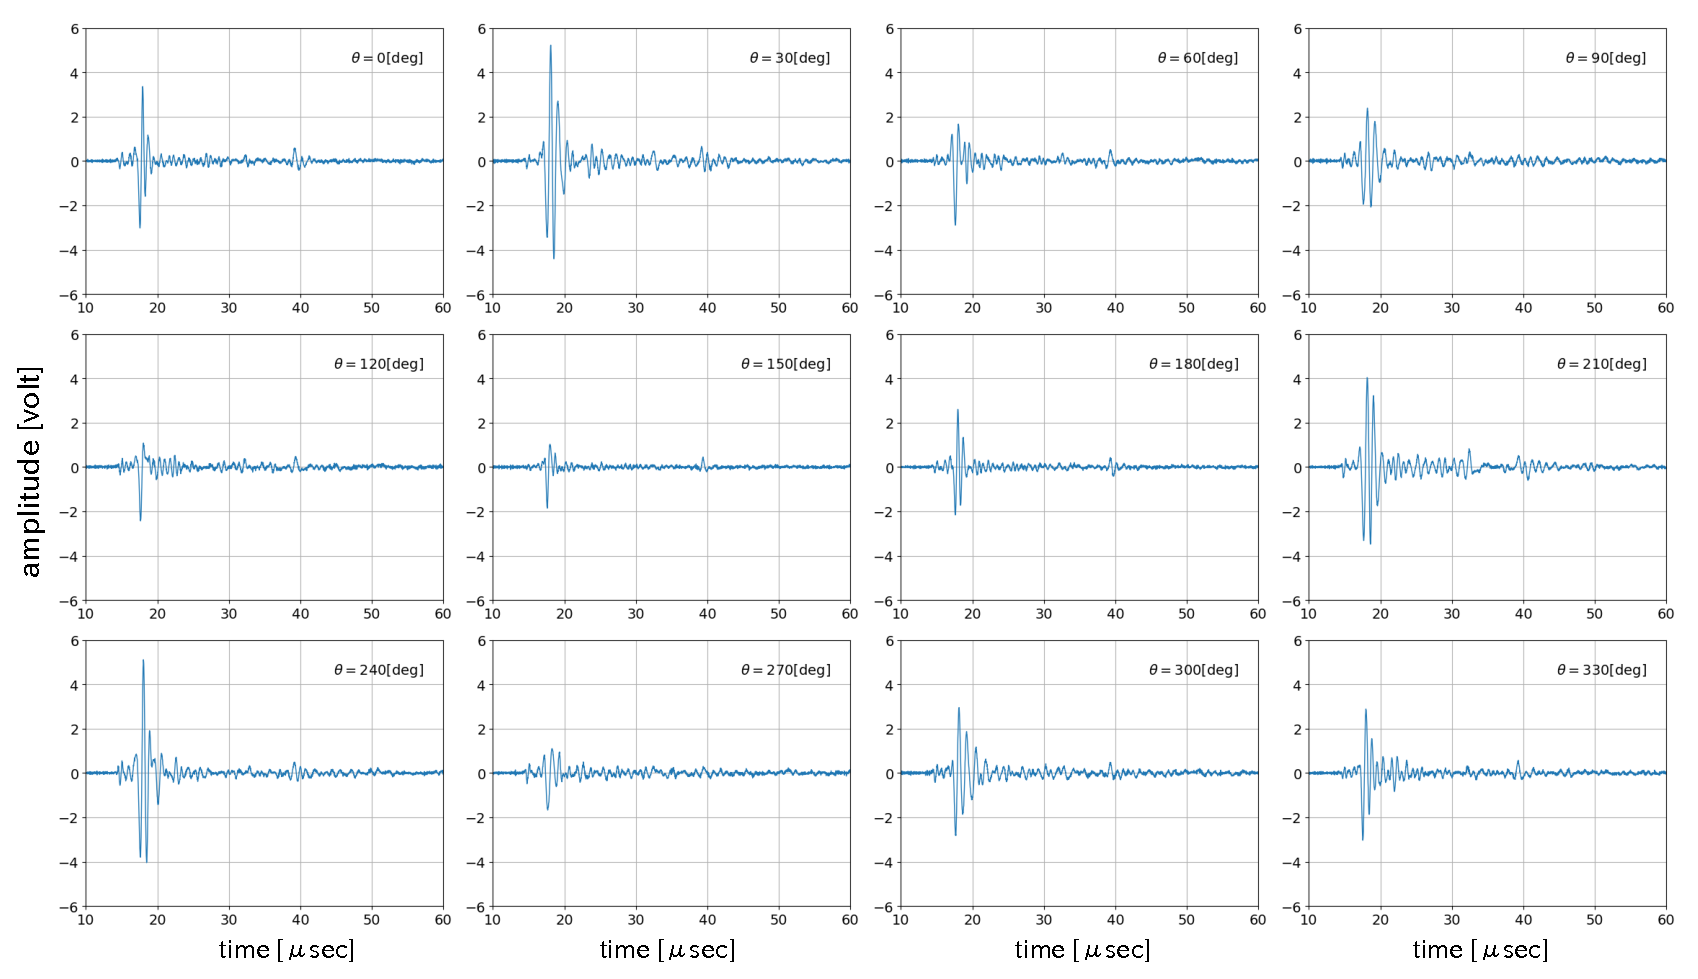
\includegraphics[width=1.0\linewidth]{Figs/fig19.eps} 
	\end{center}
	\caption{
		測線毎に算出した平均波形.
	} 
	\label{fig:fig19}
\end{figure}
%--------------------
\begin{figure}[h]
	\begin{center}
	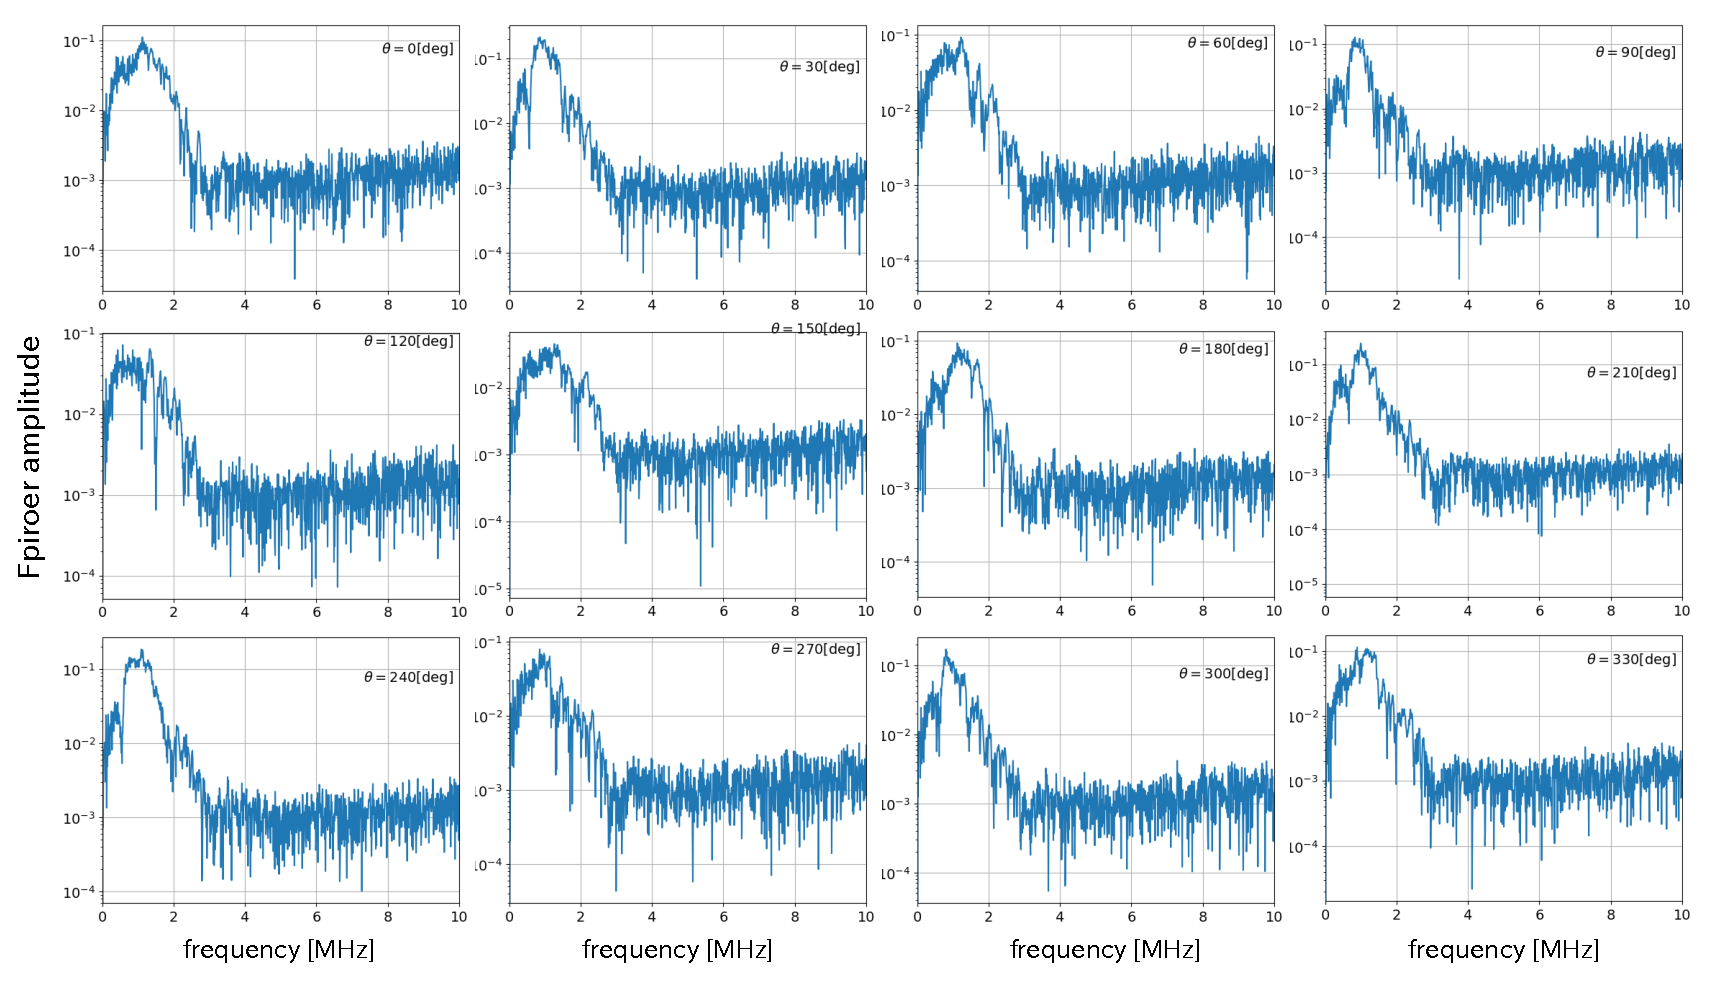
\includegraphics[width=1.0\linewidth]{Figs/fig20.eps} 
	\end{center}
	\caption{
		測線毎に算出した平均波形の周波数スペクトル.
	} 
	\label{fig:fig20}
\end{figure}
%--------------------
